\section{Experiments}
\label{sec:experiments}

% \subsection{Datasets and Metrics}

We experiment our methods on datasets with corresponding ontologies to verify the effectiveness of either ontological or temporal knowledge alone, and their combination.

\textit{AudioSet} is a large-scale multi-label audio tagging dataset collected from Youtube videos with the annotations of 527 categories out of the 632 tags defined in the ontology. Most recordings are processed into 10 seconds single-channel 16kHz, 16-bit wave format. Due to the changes of videos, it is not possible to recover the whole dataset. We downloaded 19,400 (87.5\%), 1,851,420 (90.7\%), and 17,756 (87.2\%) recordings for the balanced train, full train, and evaluation set, respectively. To simulate the low-resource scenario, we randomly sample 1\% of the unbalanced set as the training set, which has 18,514 samples, where 134 classes have no more than 5 samples, and 10 classes have no training sample. We also sample 5\% and 10\% sets for comparison. We use the commonly used mAP, mAUC as the evaluation metrics. 
\textit{SONYC} is the multi-label Urban Sound Tagging dataset used in DCASE 2019 Task5 (D19T5). It contains 2,351 train recordings and 443 validate recordings, which can be considered relatively low-resource. All recordings are 10 seconds single-channel 44.1kHz, 16-bit wave format. We use the official metrics, micro AUPRC and macro AUPRC.

\subsection{Experimental Setup}

\paragraph{Audio Features} For SONYC, we adopt a similar setting as \citep{kong2019cross}, all audios are re-sampled to 32 kHz and 64-Mel-bin log-Mel spectrograms are used to to represent the audios. The window size is 1024 samples, the hop size of 500 samples, and cut-off frequencies of 50 Hz to 14 kHz. 
For AudioSet, our setting is similar to \citep{kong2020panns}, all audios are re-sampled to 16 kHz and represented as 64-Mel-bin log-Mel spectrograms. The window size is 512 samples, the hop size of 160 samples, and cut-off frequencies of 50 Hz to 8 kHz.

\paragraph{Models and Baselines} We adopt standard CNN models as our baseline, that is, the CNN9 model use in \citep{kong2019cross} for SONYC and the CNN14 (16kHz) in \citep{kong2020panns} for AudioSet. We also introduce the SOTA method AT-GCN \citep{wang2020modeling} as baseline, which is based on co-occurrence graph mined from the whole AudioSet annotation, and uses tuned, dataset-specific hyperparameter for edge thresholding and smoothing. It is thus not directly applicable to SONYC. Our models include GCN(ASER), GCN(AudioSet), GCN(ASER+AudioSet), which refers to single GCN with temporal knowledge, AudioSet ontology, and their combination. D-GCN denotes double-GCN with 2 types of knowledge. We replace AudioSet with SONYC's ontology (OT) for experiments on SONYC dataset. We use batch size of 32 for all models and the learning rate is 1e-3 for all models except D-GCN using 3e-4.

\subsection{Results}

\subsubsection{AudioSet}


\begin{table}[tbp]
  \setlength{\belowcaptionskip}{-0.cm}
  \centering
  \small
  \begin{tabular}{lcccc}
      \hline
      {} & \multicolumn{2}{c}{Balance} & \multicolumn{2}{c}{Unbalance (100\%)} \\
      \cline{2-3}\cline{4-5} 
      Methods & mAP & mAUC & mAP & mAUC \\
      \hline
      CNN14 & 0.2441 & 0.8930 & 0.4090 & 0.9669 \\
      \hline
      AT-GCN & 0.2510 & 0.9278 & 0.4095 & 0.9664 \\
      GCN(ASER) & 0.2500 & 0.9283 & 0.3994 & 0.9660 \\
      GCN(AudioSet) & 0.2543 & \textbf{0.9420} & 0.4063 & 0.9665 \\
      GCN(ASER+AudioSet) & 0.2490 & 0.9277 & 0.3999 & \textbf{0.9690} \\
      D-GCN & \textbf{0.2554} & 0.9377 & \textbf{0.4109} & 0.9648 \\
      \hline
  \end{tabular}
  \caption{\label{tab:bal-unbal} Results on AudioSet evaluation set with models trained on balanced and unbalanced set.}
\end{table}

\begin{table}[tbp]
  \setlength{\belowcaptionskip}{-0.cm}
  \centering
  \small

  \begin{tabular}{lccc}
      \hline
      Methods &     1\% &     5\% &    10\% \\
      \hline
      CNN14                 & 0.1118 & 0.2343 & 0.2770 \\
      \hline
      AT-GCN                & 0.1243 & 0.2331 & 0.2785 \\
      GCN(ASER)             & 0.1252 & 0.2269 & 0.2735 \\
      GCN(AudioSet)         & 0.1280 & 0.2336 & 0.2747 \\
      GCN(AudioSet+ASER)    & 0.1214 & 0.2283 & 0.2741 \\
      D-GCN  & \textbf{0.1283} & \textbf{0.2387} & \textbf{0.2799} \\
      \hline
      D-GCN rel. improvement & 14.73\% & 1.88\% & 1.05\% \\
      \hline
  \end{tabular}   
  \caption{\label{tab:low-resource-map} mAP for each model trained on different portion of the unbalanced set, and the relative improvement(\%) of D-GCN over CNN14 backbone.}
  \vspace{-4mm}
\end{table}


\tabref{tab:bal-unbal} shows the performance of models trained on the official balanced and unbalanced set, while \tabref{tab:low-resource-map} shows the results on sampled subsets. We can see that all GCN-based models significantly outperform the baseline CNN14 on balanced and low-resource (1\%) set, suggesting the usefulness of the knowledge sources including the newly proposed temporal knowledge in low-resource scenarios. As the size of training data grows, the advantage of GCN models ceases to exist, expect for AT-GCN, possibly due to its knowledge of the co-occurrences on the whole training set, which matches more with the larger training data. D-GCN performs consistently better than single GCN with one KG or the simple addition of both KGs, showing the effectiveness of the separate relation modeling, and it also outperforms CNN14 by mAP in all settings despite the diminishing gain.

To study the reason for the effectiveness of GCN models in low-resource scenario (1\% set) and their degeneration in large-data settings, we divide the classes into groups according to the numbers of training samples, and calculate D-GCN's improvement over baseline on these groups. From Figure \ref{fig:delta_map_auc}, we can see that D-GCN can benefit classes with extremely few samples ([0, 5]), and the gain is the highest on classes with moderate number of samples, but not on the most prevalent classes. We may conclude that the prior knowledge in KG can effectively help the model learn the dependency between labels especially for the few-shot ones. However, as we have more resources, the large backbone model may be capable of learning such relations without KG, which explains why the advantage of GCN-based models would shrink.   

\begin{figure}[htbp]
\setlength{\abovecaptionskip}{0.cm}
\setlength{\belowcaptionskip}{-0.5cm}
\centering
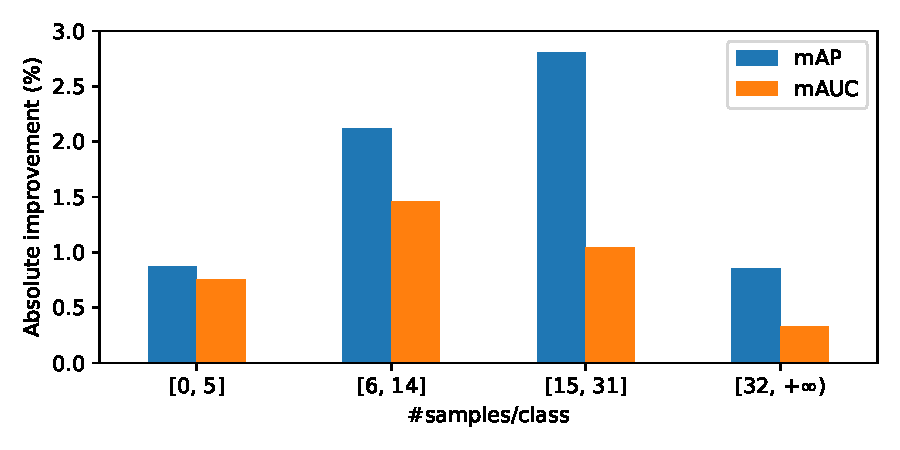
\includegraphics[width=0.9\linewidth]{figures/1p_delta_map_auc.pdf}
\caption{Absolute improvement of D-GCN over CNN14 on classes with different number 
of training samples.}
\label{fig:delta_map_auc}
\end{figure}

\subsubsection{SONYC}

\begin{table}[tbp]
  \setlength{\belowcaptionskip}{-0.cm}
    \centering
    \small
    \begin{tabular}{lcccc}
        \hline
        {} & \multicolumn{2}{c}{Fine-level} & \multicolumn{2}{c}{Coarse-level} \\
        \cline{2-3}\cline{4-5} 
        Methods & Mi AUPRC & Ma AUPRC & Mi AUPRC & Ma AUPRC \\
        \hline
        CNN9 & 0.675 & 0.493 & 0.808 & 0.580 \\
        GCN(ASER) & 0.703 & 0.459 & 0.822 & 0.548 \\
        GCN(OT) & 0.680 & 0.494 & 0.821 & 0.596 \\
        GCN(ASER+OT) & 0.706 & 0.492 & \textbf{0.823} & 0.616 \\
        D-GCN & \textbf{0.709} & \textbf{0.516} & 0.820 & \textbf{0.647} \\
        \hline
    \end{tabular}
    \caption{\label{tab:SONYC} Results on SONYC validate set, OT: SONYC ontology, Mi: Micro, Ma: Macro.}
    \vspace{-4mm}
  \end{table}

The results on the SONYC dataset is shown in Table \ref{tab:SONYC}. Similar to AudioSet (1\%), all GCN models significantly outperform baseline by the main metric Micro AUPRC. The temporal knowledge of ASER seems to be more useful here compared to ontology, as the ontology for SONYC is more sparse, and the labels for each level are predicted separately, so that they don't co-occur. D-GCN again gives consistently best or competitive performance on both level, suggesting the generalizability of this method on effectively combining the strength of two knowledge types.
